\documentclass{bmvc2k}

%% Enter your paper number here for the review copyu
\bmvcreviewcopy{666}

\title{Correspondence matching of non-coplanar circles from a single image}

% Enter the paper's authors in order
% \addauthor{Name}{email/homepage}{INSTITUTION_CODE}
\addauthor{Susan Student}{http://www.vision.inst.ac.uk/~ss}{1}
\addauthor{Petra Prof}{http://www.vision.inst.ac.uk/~pp}{1}
\addauthor{Colin Collaborator}{colin@collaborators.com}{2}

% Enter the institutions
% \addinstitution{Name\\Address}
\addinstitution{
 The Vision Institute\\
 University of Borsetshire\\
 Wimbleham, UK
}
\addinstitution{
 Collaborators, Inc.\\
 123 Park Avenue,\\
 New York, USA
}
\usepackage[]{algorithm2e}

\runninghead{Student, Prof, Collaborator}{BMVC Author Guidelines}

% Any macro definitions you would like to include
% These are not defined in the style file, because they don't begin
% with \bmva, so they might conflict with the user's own macros.
% The \bmvaOneDot macro adds a full stop unless there is one in the
% text already.
\def\eg{\emph{e.g}\bmvaOneDot}
\def\Eg{\emph{E.g}\bmvaOneDot}
\def\etal{\emph{et al}\bmvaOneDot}

%------------------------------------------------------------------------- 
% Document starts here
\begin{document}

\maketitle

\begin{abstract}
In this work we have proposed a method to determine 2D-3D correspondence between non-coplanar circles from a single image.
Our method uses image conics to compute circle plane orientation in camera coordinate system, thus bringing the problem from 2D to 3D domain. This information is used to generate projective invariant descriptors which can be used directly for correspondence matching, given that the 3D information about circles are known. Additionally, the evaluation also covers study stability of the projective invariants and the factors affecting their computation. One of the intended applications is for tracking industrial objects with circles on it. In our approach we use conic properties of circles to compute projective invariant descriptors. These descriptors are matched with known 3D information to establish correspondences. We also demonstrate stability of the invariants used to generate descriptors both in practice and simulation. 
In our approach we compute 3D plane orientation of each circle from its image contour, and compute projective invariants between each pair of circles. We propose a new descriptor 

\end{abstract}

%------------------------------------------------------------------------- 
\section{Introduction}
\label{sec:intro}
goal : 
Explain the problem in question, the motivation for the work and the proposed application in mind. The assumptions made in our work. We have the camera calibrated and we use 3D points and their normal positions for the descriptor measurement. 
%No much work done in this direction. The invariants proposed are never used for a application so we provide use and discuss stability of the algorithm. Comment on why circles and the paper we build up to. 
%The work of Forsyth as the base of our work, the concepts given in the paper. Our contribution is matching strategy using such invariants. Demonstrating an application and evaluation of the method. 

Correspondence matching is one of the key problems in computer vision. Applications related to pose estimation or object detection require accurate knowledge of model features and their corresponding image features. 
The problem becomes more challenging for monocular systems as the depth information is lost. Popular monocular methods involve learning object with few initial frames or require initialisation to facilitate matching [N3M so on]. Many authors have proposed using natural features like points, lines and conics for solving correspondence problem \cite{hartley_multiple_2003}. Such features are easier to extract from images and can be used to compute reliable projective invariants. Invariants are extensively studied topic in early vision community, Forsyth \etal \cite{forsyth_91} provided a detailed account on 3D invariant descriptors and their stability under projective motion. 
In learning based model tracking methods initial frames of the camera are used to learn model and compute unique descriptors from dense or sparse set of natural model features \cite{chekhlov_ninja_2007} \cite{hinterstoisser_n3m:_2007} \cite{lowe_object_1999}. Other methods involve using a selective set features (edges, contours, etc.) to compute invariants from a single image \cite{lepetit_monocular_2005}. In our method we demonstrate how non-planar circular features can be used to compute invariant descriptors and solve matching from single image. 
%We propose one such method for multiple non-coplanar circular features exist in the scene. solving correspondence problem when 
%Machine learning based methods \cite{Hartley00} provide promising results, but are limited to a specific group of objects and require prior learning of the object. 
%This work is focussed on finding correspondence information from a single image of the scene. 
%Methods [quan] find correspondence    

%Many authors have proposed using natural features like points, lines and conics for solving correspondence problem. 
%The core idea is to compute projective invariants from such features to obtain robust matching with model feature points.
%[Quan] One approach is using two or more images from different perspective to find same image features and then obtain correspondence using triangulation technique. 
%The problem is more complex with a single image as depth feature is lost. 
%In this paper we will focus on solving this particular problem of matching from a single image. 

In single images projective transformation of features make it difficult to compute invariant features. Coplanar conics, lines and points can be used to compute planar invariants \cite{forsyth_91}. Circles have a special property to retain depth information under projective transformation. A world circle always produces an elliptical curve on the image plane. If size of circle is known orientation of circle plane can be defined in 3D (camera coordinates) with a two fold ambiguity \cite{forsyth_91} \cite{safaee-rad_three-dimensional_1992}. 
Further, Forsyth \etal \cite{forsyth_91} proposed that up to three projective invariant can be computed from a non-coplanar pair of circles. They explain that angle between circle planes (angle between surface normals) and distance between centre of the circles are invariant quantities. The concept was proposed in early 90s, however these invariants have remained unexplored. 
We propose using these invariants to solve correspondence problem when multiple 3D circular features exist on a model. 
In this approach we bring problem from 2D to 3D by computing 3D invariants from image features, then solve 3D-3D matching problem with model. (Fig of decsriptor match) 
We use invariant descriptors (computed from elliptical image features) to solve the conic ambiguity and provide accurate matching with 3D features. 
The proposed method is first attempt to use these invariants, therefore we also carried out simulations to show stability of invariants against change of perspective.  

%We demonstrate  practical scenario where such method can be used effectively.
Our contribution is a new method to accurately identify image correspondences when multiple identical 3D circular features exist in the scene. We assume that calibration of camera is known and 3D information of features is available. 
Often in Industry based model tracking applications 3D-CAD data is known. Our matching method is suitable for tracking any 3D objects having known circles on different planes. In close range photogrammetry multiple circular markers (fig) are placed on 3D models for surface measurements \cite{luhmann_close_2006}. 
These measurements include computation of surface normal and 3D position of each marker. 
This process involves taking multiple images of the model with additional presence of encoded markers in the scene to solve correspondence. 
Once 3D measurements are done our method can be extremely useful to support tracking application without using coded patterns. Similarly various industrial parts having natural circles can be identified and tracked with this method. 
We prepared two car models with circular markers for evaluating our matching method. The proposed method can find corresponding circular marker from a single image, with high accuracy. We also show that our method is stable against false positives detected from the scene. Our method is fast enough to support real-time tracking applications. 

[REFER : Comment on descriptor being propose of 3D point an normal based info. ]

%-> Figure explaining the issue 
%\begin{figure}
%\begin{tabular}{ccc}
%\bmvaHangBox{\fbox{\parbox{2.7cm}{~\\[2.8mm]
%\rule{0pt}{1ex}\hspace{2.24mm}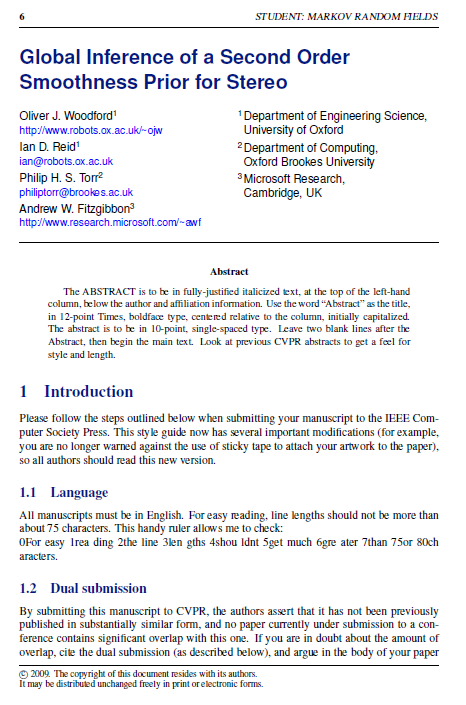
\includegraphics[width=2.33cm]{images/eg1_largeprint.png}\\[-0.1pt]}}}&
%\bmvaHangBox{\fbox{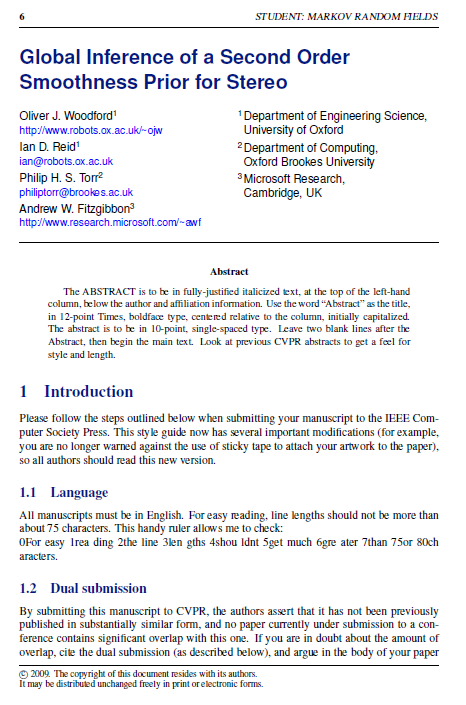
\includegraphics[width=2.8cm]{images/eg1_largeprint.png}}}&
%\bmvaHangBox{\fbox{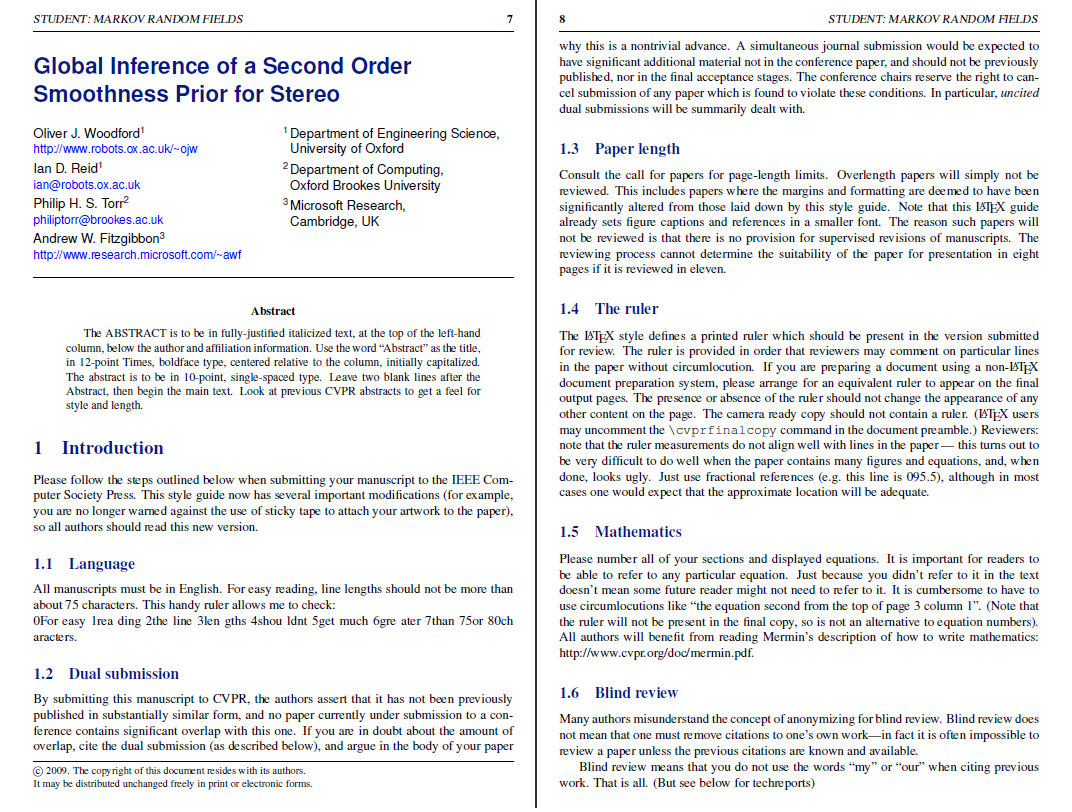
\includegraphics[width=5.6cm]{images/eg1_2up.png}}}\\
%(a)&(b)&(c)
%\end{tabular}
%\caption{It is often a good idea for the first figure to attempt to
%encapsulate the article, complementing the abstract.  This figure illustrates
%the various print and on-screen layouts for which this paper format has
%been optimized: (a) traditional BMVC print format; (b) on-screen
%single-column format, or large-print paper; (c) full-screen two column, or
%2-up printing. }
%\label{fig:teaser}
%\end{figure}

\section{Related Work}

Object detection and pose estimation from conic features is widely studied in 3D vision literature  \cite{dhome_spatial_1990}\cite{safaee-rad_three-dimensional_1992} \cite{werghi_pose_1996} \cite{quan_invariant_1995}. Circular shape is also a popular choice for designing artificial fiducial. Detection of contour points from image and fitting ellipse is a well studied topic \cite{fitzgibbon_direct_1999}. 
%Detection of conic sections from the image is easy and also a widely studied subject [conic fitting, gibbon].
Quan \cite{quan_conic_1996} proposed a two view approach for finding correspondence and 3D reconstruction with conic section. Authors have proposed methods to compute invariants for coplanar conics \cite{forsyth_91} \cite{Ferri_1993}.  
%Various tracking and camera calibration methods use a pair coplanar circular features to compute invariant descriptors. 
A 3D problem is simplified to 2D when coplanar features are recovered and used for correspondence.  
Ying \etal \cite{ying_camera_2007} use a coplanar pair for camera calibration. 
Uchimaya \etal \cite{uchiyama_random_2011} developed invariant descriptors from multiple coplanar circles, and extended the work for deformable model \cite{uchiyama_deformable_2011}.
Work of \cite{lo_pez_de_ipin_a_trip:_2002} \cite{naimark_circular_2002} \cite{pagani_circular_2011} propose a circular marker for 6D pose estimation, no invariants are computed as correspondence is solved by using unique coded pattern around the circle. 
\cite{lo_pez_de_ipin_a_trip:_2002}\cite{pagani_circular_2011} use circular shape to define circle plane in 3D, Additionally use a coded pattern is used encode 6D pose without ambiguity.(Fig). 
Luhmann \cite{luhmann_close_2006} provides detailed account of methods using point circular fiducials in close range Photogrammetry. The current state of the art methods coded patterns are introduced to simplify correspondence problem.
[GOM][AICON] are one of the industrial supplies for close range photogrammetry measurement equipments. 

[Refer Thesis: Comment on catalogue based methods, ]
\paragraph{}
Literature study suggests that, existing methods either provide a solution for coplanar circular features or non-coplanar  coded circular features. The novelty of our method is that it addresses 2D-3D matching problem for non planar circles present in the scene. 

\section{Method}
We assume that both 2D and 3D data is already available, and will focus on the matching method in detail. 
3D data includes the surface normal ($N_i$), centre position ($M_i$) and size ($R_i$) of the circles on the model. 
2D data includes centre points ($m_i$) and conic matrices ($C_i$) recovered from the undistorted image. The camera intrinsics ($K$) and distortion parameters are known. We have followed approach of Naimark \cite{naimark_circular_2002} and Fitzgibbon \cite{fitzgibbon_direct_1999} for ellipse detection and fitting.  

\subsection{Conic Invariants : Theory and Computation}
\label{subSec:ConicInv}
In this part we will explain the theory and computational aspect euclidean invariants computed from the image.  
%The invariants generate by a pair of non-planar circles is explained by Forsyth \etal \cite{forsyth_91}. 
If camera's projection centre is assumed as the vertex of a cone which has the world circle is at its base.
The image plane can be considered as a cutting plane $\pi$, which always creates an elliptical cross section.  
%Theory of conic sections can be used to suggest that the image projections are nothing but a cross section of a cone. 
A new plane $ \pi' = T* \pi $ can be computed such that intersection of plane $\pi'$ with the cone is circular. 
%A rotation transformation $T$ can be applied to the image plane such that the intersection of transformed plane $\pi'$ with the cone is a perfect circle. 
Plane ($\pi'$) is parallel to the base of the cone hence a plane normal $Nc_i$ can be computed from $T$. 
Additionally, 3D position of circle centre $Mc_i$ can be computed in camera coordinate system if original radius is known.
A normal $Nc_i$ and a point on plane $Mc_i$ are sufficient to define the plane of circle in camera coordinate system.
$ T $ is a combination of two rotations \cite{forsyth_91}\cite{lo_pez_de_ipin_a_trip:_2002}, one of the two has $\pm \phi$ rotation angle which introduces the ambiguity (two solutions) in plane recovery. 
This implies that every image conic results in to two possible plane orientations, we call this method as Ellipse Backprojection. 
\begin{equation}
\text{Ellipse Backprojection}(m_i,C_i) \rightarrow {Nc_i}^1,{Nc_i}^2,{Mc_i}^1,{Mc_i}^2
\end{equation}
Forsyth \etal \cite{forsyth_91} explained that for three dimensional objects descriptors consist of euclidean invariants rather than projective invariants. Three type of \textit{Conic invariants} can be computed from a pair of non-coplanar circles.
We use following invariants for our method, 
\begin{enumerate}
	\item \textbf{Angle between planes} ($\theta$) : It is same as angle between their surface normals 
	(i.e. $ \angle(Nc_i,Nc_j) $). $\theta$ can be recovered from conic image without knowledge of circle size in real world.  
%	\item \textbf{Ratio of circle radius to distance between circle centers}: This invariant can also be recovered without radius value.
	\item \textbf{Distance between circle centres} : This vector $ V $($ Mc_i,Mc_j $) has three degrees of freedom. The length of the vector $d_c$ is invariant (object scale should be known) and consistent despite of the ambiguity. 
\end{enumerate}
It should be noted that ambiguity of Ellipse Backprojection produces 4 solutions for $\theta$, only one of which is correct. 
Other invariants can be computed from recovered normal and centre values. These invariants are unstable \cite{forsyth_91} as the error from both recovered components influences the computation.
The quality of Ellipse Backprojection depends on distance from the camera and the viewing angle (angle between the image plane and the circle plane)\cite{werghi_pose_1996}. 
We performed simulations for circles of diameter ($\phi$) of 5,8,12 mm to understand behaviour of Ellipse Backprojection on small features. We varied the camera distance (0.5 to 2 m) and viewing angle (0-70$^\circ$) in step wise manner, while recording 100 iterations at each step.
At low viewing angles 0-10$^\circ$ both angle and centre recovery has higher errors, at any fixed distance. 
The shape of ellipse is almost circular at small viewing angles, this factor can explain high errors. 
Error in estimation grows with camera distance, however normal recovery appears less sensitive to camera distance than centre recovery. We can conclude that normal recovery has less errors but computation of $\theta$ will result in 4 solutions. The comparison of the ambiguity explains that estimated centres are very close to each other ($ d({Mc_i}^1,{Mc_i}^2) \leq$ 0.1 mm for $\phi$= 12 mm), therefore any one of the solutions can be chosen. The centre recovery is prone to higher errors, however has a unique solution (all 4 solutions are consistent).

\subsection{Descriptor Generation}
This part mainly discusses generation of \textit{Conic descriptor} from computed invariants. 
Invariants for model points can be computed from available 3D data ($M_i,N_i$) without any ambiguity. 
The same set of invariants can be computed a single 2D image using Ellipse backprojection with Conic ambiguity.
In our approach we pursue the idea that existence of multiple features can be used to overcome the Conic ambiguity problem. 
The principle idea is to generate unique descriptors from Conic invariants to perform a direct matching.
We propose \textit{Conic Descriptor} which also encapsulates the conic ambiguity, 
\begin{align}
\textit{Conic Descriptor}_{image} &= v_{q} \langle  d_c,\theta_{11},\theta_{12},\theta_{21},\theta_{22} \rangle_{i,j} \\
\textit{Conic Descriptor}_{model} &= V_{p} \langle d_c,\theta \rangle_{i,j}
\end{align}
where $v_{q}$ represents image conic pair $i,j$ and $V_{p}$ represents world circles $i,j$. 
PFH descriptors \cite{RusuDoctoralDissertation} show similar descriptor structure, input 3D point and normal information is without an ambiguity. 
Unlike popular methods \textit{Conic Descriptor} is designed to represent two features at same time. 
A descriptor to represent a single conic requires using at least more than two conic features. 
Each conic adds 3 wrong solutions of $ \theta $, additionally matching must rely on detection of all conics used for descriptor computation.
As correspondence is not available $ v_{\{1..q\}} $ are computed for all $ n $ image conics, where $ q = \binom{n}{2} $. 
%In our method $ q = \binom{n}{2}$ \textit{Conic Descriptors}($ v_{\{1..q\}} $) are generated for n image conics. 
$ V_{\{1...p\}} $ are computed off-line as the 3D data is already available. In this case for $ l $ world circles  $ p \leq \binom{l}{2} $, as pairs not likely to appear in same image can be rejected. After computing Conic descriptors from image following 3 step matching process is used to achieve 2D-3D correspondences. 

% -> Figure explaining the issue
%\begin{figure}[!ht]
%\centering
%\subfloat[A problem showing four image points, and their correspondence with world points (1-A,2-B,C-3) and one false positive (D)\label{fig:matchingProblem} ]
%{\includegraphics[width = 0.45\textwidth ]{images/matchingProblem.png} }
%\subfloat[Image shows the simplified matching process for the problem suggested in (a), partial results of all 3 steps are shown. \label{fig:matchingProcess}  ]
%{\includegraphics[width = 0.45\textwidth]{images/matchingProcess.png} }
%\caption{Matching problem and the overview of the method to generate correspondence hypothesis :\label{fig:matchingAndProblem}}
%\end{figure}

\begin{figure}
\centering
\begin{tabular}{cc}
\bmvaHangBox{\fbox{\includegraphics[width=5cm,keepaspectratio=true]{images/matchingProblem.png}} }&
\bmvaHangBox{\fbox{\includegraphics[width=5cm,keepaspectratio=true]{images/matchingProcess.png}} } \\
%\caption{\label{fig:matchingProblem}}
%\caption{\label{fig:matchingProcess}}
(a)&(b)
\end{tabular}
\caption{ Matching problem and the overview of the method to generate correspondence hypothesis ;
(a) A problem showing four image points, and their correspondence with world points (1-A,2-B,C-3) and one false positive (D) (b) Image shows the simplified matching process for the problem suggested in (a), partial results of all 3 steps are shown. \label{fig:matchingAndProblem}}
\end{figure}

\subsection{Step 1: Pairwise Initial Matching}
\label{subSec:PIM}
In the first stage of matching process we find a possible conic pair correspondence ($ V \leftrightarrow v $).
The objective is to reduce complexity of the problem by finding possible correspondence candidates. 
The strategy is to first compare unique component($ d_c $) of descriptors, if positive then check for ambiguous component ($ \theta $) for a possible match against all 4 values. 
$ T_{d_c} $ and $ T_\theta $ are the thresholds used to compare the components. 
The stage may result in \textit{one to many} type of relation between descriptors. This can be either due to similar feature orientation on object or due to presence of \textit{Conic ambiguity} (ambiguous $ \theta $ solutions). 
The reader should note that a descriptor represents a pair of conics, therefore even an accurate match does not solve individual correspondence in this stage. 

\begin{algorithm}
\SetKwData{threeDFv}{$ V_{p} $}\SetKwData{twoDFv}{$ v_{q} $}
\SetKwData{ThresholdD}{$T_{d_c} $}\SetKwData{ThresholdA}{$T_\theta $}
\SetKwFunction{compareDist}{compare$d_c$}\SetKwFunction{compareAngle}{compare$ \theta $}
\SetKwFunction{Save}{SavePairResult}
\emph{Goal : Find all possible \threeDFv similar to \twoDFv} \;
\emph{Initialisation : \ThresholdD = 10 , \ThresholdA = 5} \; 
\ForAll{ 3D Feature Descriptors ($ V $), $ p \leftarrow 0 $ \KwTo $ n $}{	
	\ForAll{ 2D Feature Descriptors ($ v $), $ q \leftarrow 0 $ \KwTo $ l $}{
			% Project conic points 
			\If (\tcp*[h] {compares $ d_c $ component} ){ \compareDist{\threeDFv,\twoDFv} $ < $ \ThresholdD } {
				\If (\tcp*[h] {compares $ \theta $ component} ){ \compareAngle{\threeDFv,\twoDFv} $ < $ \ThresholdA }{
				\tcp{ All 4 solutions of $ \theta $ in $ v_q $ are checked } \;			
				\Save{$ p,q $} \tcp{Save matching descriptor pair} \;
				}
			}
		}	
	}
\caption{Initial pair matching algorithm}
\end{algorithm}

%------------------------------------------------------------------------- 
\subsection{Step 2: Pointwise Triplet Matching}
In this stage we simplify the problem further and obtain point wise matching ($ m_i \leftrightarrow M_i $) by performing a verification on $ v \leftrightarrow V $ matching results. 
The first objective is to identify and reject false descriptor matches, thereby obtaining a \textit{one to one} conic pair matching relation. Additionally, a single conic pair matching still leaves ambiguity regarding individual conic correspondence $ m_i \leftrightarrow M_i $. 
We follow a two step approach to generate a matching hypothesis,
\begin{enumerate}
\item[1] Find any two results of Pairwise matching in which both image and model descriptors represent one and only one common conic. If such results exist then an initial triplet matching hypothesis can be proposed.
\[
 V_{12} \leftrightarrow v_{AB},V_{13} \leftrightarrow v_{AC } \xrightarrow{\text{Triplet Hypothesis}} [1~2~3] \leftrightarrow [A~B~ C]
\]
In the example above we can see that world conic 1 and image conic A is common among two solutions. We form a 3 point matching hypothesis with these results. 
\item[2] Find a new descriptor matching pair ($ V_{23} \leftrightarrow v_{BC}$) which can verify the 3 point matching hypothesis.
\end{enumerate}
If a triplet is verified then the result is saved for further processing. This step may also contain false triplet matches (Ref. \ref{fig:matchingAndProblem}). 

\subsection{Step 3: Correspondence Hypothesis }
\label{subSec:CHypo}
In this final step results of Pointwise Triplet matching are combined and a voting matrix is generated (Ref. \ref{fig:matchingAndProblem}). A pair having maximum votes in the matrix is proposed as a correspondence hypothesis. In case of conflicting votes results are not considered. A minimum of 3 correspondence are required to compute the pose of the object \cite{lepetit_monocular_2005}(camera intrinsics are known). We recommend computing pose of the object by 
selecting top 3 correspondence results. The computed pose can be used to further verify and modify correspondences. This implies that for images having only 3 conic features matching results may not be reliable. 

%\begin{figure*}
%\begin{center}
%\fbox{\rule{0pt}{2in} \rule{.9\linewidth}{0pt}}
%\end{center}
%   \caption{Example of a short caption, which should be centered.}
%\label{fig:short}
%\end{figure*}

%\begin{table}
%\begin{center}
%\begin{tabular}{|l|c|}
%\hline
%Method & Frobnability \\
%\hline\hline
%Theirs & Frumpy \\
%Yours & Frobbly \\
%Ours & Makes one's heart Frob\\
%\hline
%\end{tabular}
%\end{center}
%\caption{Results.   Ours is better.}
%\end{table}

\section{Evaluation}
In this section we will cover experiments (simulations and real) carried out to comment on accuracy and robustness of the algorithm. To the best of our knowledge no other application has attempted using the euclidean invariants generated by circles. 
The reader should note that the problem of achieving single image correspondence with non-coplanar circles is not addressed earlier. Therefore, alternative methods for comparison are not available. 
We prepared a test scenario by attaching uncoded circular markers of size $ \phi $ = 12 mm ($ M_i = 20 $) and 5mm ($ M_i  = 26$) to two identical car models.  
The markers are attached randomly and coplanar placement is avoided.
Measurement of 3D data is done with state of the art metrology systems, and ground truth is established by giving each model point a unique ID in database. 
Images of the models are captured from different perspective with a calibrated camera (5 Mpx). 

\subsection{Experiment 1 : Descriptor Matching vs Marker Orientation}
This experiment is carried out to understand the factors affecting descriptor matching stage with respect to orientation of the circles.
A MATLAB simulation is performed to position two circles in different orientations and captured images (noise $ \sigma = 0.3 $) from 1000 different camera positions for each orientation.  
%(Rotation angles : -65 to 65, X-Y Translation : -100 to 100 ).
The control parameters are distance between circle centres ($ d_c $) is varied from 10 - 150 and plane angle ($ \theta $ )is varied from 10 - 90. Realistic values are used for camera intrinsics, $ T_{d_c} $ = 10 and $ T_\theta $ = 5 are kept constant through the experiment. Rotation ($ R $) and Translation ($ T $) parameters for camera position are random, only $ T_z $ parameters is limits are different from smaller and bigger markers. 

\begin{table}
\centering
\caption{Descriptor Matching Analysis } \label{table:MatchingSuccess}
\begin{tabular}{|c| c | c | c |}
\hline
$ \phi $ & $ \theta $ & Camera Distance (mm) & Matching Success($ \% $) \\ \hline
12 & 0-40 & 500-2000 & 80-95 \\
& 40-90 & 500-2000 & 50-80 \\
& 0-40 & 2000-4000 & 40-60 \\
& 40-90 & 2000-4000 & 20-40 \\ \hline
5 & 0-40 & 500-1200 & 75-90 \\
 & 40-90 & 500-1200 & 40-75 \\
 & 0-40 & 1200-2000 & 55-80 \\
 & 40-90 & 1200-2000 & 35-55\\ \hline
 20 & 0-80 & 500-2000 & 100 \\
 20 & 80-90 & 500-2000  & 30-90 \\ \hline 
\end{tabular} \\
\label{tab:Exp1}
\end{table}
The table above provides summary of key observations of the experiment. Matching result shown is AND operation between $ d_c $ match and $ \theta $ match ( Sec. \ref{subSec:PIM}). 
% (Success vs $ d_c $ vs $ \theta $) 
The key learning from this experiment is that descriptor matching is influenced more by angle between planes than distance between circles at fixed threshold values. It is also seen that success of matching can be improves significantly with increased size of circles, even at higher values of $ \theta $. This experiments suggest that when features placement is possible in scene it is advised to chose larger circles or surfaces with lower plane angles for better matching. 

%------------------------------------------------------------------------- 
\subsection{Correspondence Matching vs Threshold Settings}
The first experiment has recommendation regarding choice of features and placement of features. In a realistic scenario this option may not be available, therefore aim of the experiment is to understand the role of threshold values ($ T_{d_c}, T_\theta $) in overall correspondence matching results. In order to perform this experiment we took 75 images of car model with 12 mm markers (Distance Range 0-2000 mm). All the results (Table.~\ref{tab:Exp2}) are verified with ground truth data manually. 
The images have at least 4 conics detected in each image. If hypothesis proposes less than 3 $ m_i \leftrightarrow M_i $ results we consider it as \textit{Not Converged}. \textit{Correct} results are divided in two categories purely to provide detailed overview of algorithm performance. \textit{ Complete} refers to $ m_i \leftrightarrow M_i $ hypothesis being 100\% correct, \textit{Partial} results suggest that some of the matching results (excluding top 3 voted pairs) are not correct.  

\begin{table}
\centering
\caption{Correspondence matching with varying threshold settings } \label{table:ThresholdEffect}
\begin{tabular}{ | c | c | c | c | c | c |}
\hline
\multicolumn{2}{|c|}{Settings} & NC & \multicolumn{2}{|c|}{Correct} & Wrong \\ \hline
$ T_\theta $ & $ T_{d_c} $ & {} & Complete & Partial & {}\\ \hline
5 & 5  & 13 & 62 & 0 & 0 \\
5 & 10 & 8 & 67 & 0 & 0 \\
5 & 15 & 4 & 67 & 0 & 4 \\ \hline
3 & 5  & 28 & 47 & 0 & 0 \\
3 & 10 & 21 & 50 & 4 & 0 \\
3 & 15 & 19 & 52 & 1 & 3 \\ \hline
\end{tabular} \\
\label{tab:Exp2}
\end{table}
In Sec. \ref{subSec:ConicInv}, we learned that $ d_c $ recovery is weak and therefore a flexible threshold may be appropriate for matching. The results ( Table. \ref{tab:Exp2}) show that flexible $ T_{d_c} $ with stringent $ T_\theta $ may allow more Pairwise matching results, but due to \textit{conic ambiguity} of $ \theta $ probability of wrong matching goes higher. 
On the other hand, very stringent thresholds lead to higher non convergence. Therefore, a right balance of threshold can be selected to achieve balanced results. Our preferred settings for experiments is $ T_{d_c} = 10 $ and $ T_\theta = 5 $, as 90\% of images show maximum 100\% success with (0\%) wrong matching. The selection may require change based on density of the features. 

\subsection{Robustness against false positives}

%------------------------------------------------------------------------
\subsection{Time Analysis}
In this experiment we focus on analysing time consumed by the matching method when introduced into a tracking application. 
Two cameras CAM 1 (2560 x 1920) and CAM 2 (640x480) are used for tracking, the results presented are averaged over 100 frames. 
The results show that our method takes $ \leq 1\% $ time from in the tracking pipeline. In terms of frame rates we achieve 2-3 FPS with CAM 1 and 7-8 FPS with CAM 2. Additionally, an exhaustive experiment with 90-140 false positives in the scene shows that matching consumes maximum time in the pipeline (0.7 FPS). Limited tracking range ($<$ 500 mm) of CAM 2 does not allow experiment with such large number of false positives. 
\begin{table}
\caption{Time Analysis}\label{table:trackPerformance}
\centering
\begin{tabular}{|c | c | c | c |}
\hline 
Algorithm Stage & \multicolumn{2}{|c|}{CAM 1} & CAM 2\\ \hline
{} & Model & Model + FP & Model \\ \hline 
Image Undistortion & 39.53\% & 12 & 11.79 \\
Marker Detection & 38.51 & 34 & 30.75 \\
Correspondence Matching & 0.35 & 44.2 & 1.34 \\
%Descriptor Generation & 0.10 & 0.33 \\
%Descriptor Matching & 0.25 & 1.01 \\
Pose Estimation & 21.61 & 9.8 & 56.12 \\ \hline
\end{tabular}
\end{table}

\section{Conclusion \& Future work }
%----------- Do I mention conic ambiguity? 
In this paper we have demonstrated a successful approach for solving 2D-3D correspondence matching problem for non-coplanar circular features from a single image. 
We propose a new \textit{Conic descriptor} which represents euclidean invariants generated by a pair of non-coplanar circles.
Our method can successfully define correspondences for more than 3 circular features are present in the scene. 
The proposed method is the first to address the correspondence matching using these invariants since its introduction in the 90s.
Our contribution also includes providing detailed understanding of behaviour of invariants with respect to orientation and size of the circles. The major factors affecting matching are also discussed to optimize the method for best possible matching results based on application (threshold settings, circle size, camera distance). 
The results of the experiments support our claim, that the method is fast, reliable and robust against false positives.
Our method can be used for object tracking or object identification in Industrial scenario, where natural or artificial circular features exist on the models. However, the method is generic and can be used for any application dealing with non coplanar circles. 
The 3D information of the features on the model and camera calibration are the only prerequisites for matching. 
The reader should also note that algorithm may not perform well with symmetric arrangement of circular features. 

In context of future work, a faster matching strategy can be developed to handle large number of feature points and false positives. We would like to use the same invariants to compute 2D-2D correspondence matching between two images in order to generate the 3D data which is a prerequisite now. We also consider using such matching algorithm to support creating 3D markers for monocular Augmented Reality applications. This can be a cheap alternative to conventionally used 3D spherical markers.  

Page 7 : 
1. Reliable method for correspondence matching for non coplananr circular features. 
2. Accuracy is improved with the size and method works better if the detection range is selected appropriate to the conic size. 
3. Comment on the stability of the invariants 
4. Comment on arrangement of the circles. (Random and non symmetric)

\bibliography{egbib}
\end{document}
